% a tikz figure for feature fusion block diagram

\usetikzlibrary{shapes}

\tikzstyle{edata}=[draw,thick,rounded corners,minimum height=1cm,text width=2cm,align=center]
\tikzstyle{data}=[above,text width=1.5cm,align=left]
\tikzstyle{process}=[rectangle,draw,thick,minimum height=1cm,text width=2cm,align=center]
\tikzstyle{fusion}=[rectangle,draw,thick,minimum height=3cm,text width=2cm,align=center]
\tikzstyle{io}=[]

\resizebox{\textwidth}{!}{
\scriptsize
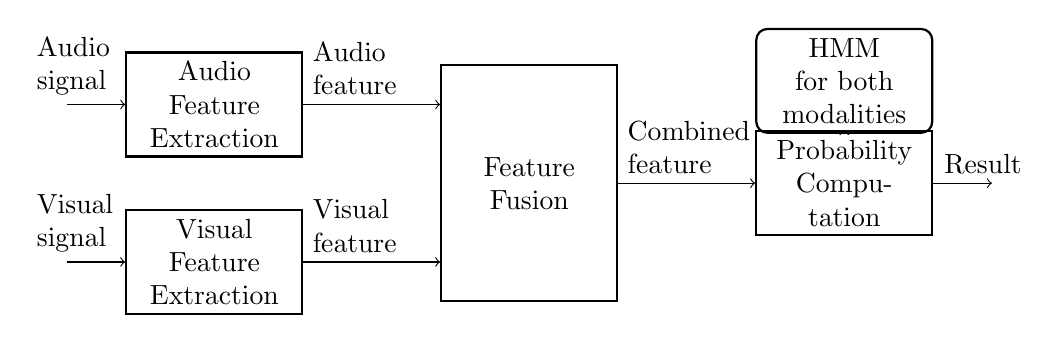
\begin{tikzpicture}
  \node[io] (iv) at (1,0) {};
  \node[process] (pv) at (3,0) {Visual Feature Extraction};
  \node[io] (ia) at (1,2) {};
  \node[process] (pa) at (3,2) {Audio Feature Extraction};
  \node[fusion] (ff) at (7,1) {Feature Fusion};
  \node[process] (cl) at (11,1) {Probability Computation};
  \node[edata] at (11, 2.3) {HMM for both modalities} edge[->] (cl);
  \node[io] (o) at (13,1) {};

  \draw[->] (iv) -- node[data] {Visual\\ signal} (pv);
  \draw[->] (ia) -- node[data] {Audio\\ signal} (pa);
  \draw[->] (pv) -- node[data] {Visual\\ feature} (pv -| ff.west);
  \draw[->] (pa) -- node[data] {Audio\\ feature} (pa -| ff.west);
  \draw[->] (ff) -- node[data] {Combined feature} (cl);
  \draw[->] (cl) -- node[data,align=right] {Result} (o);
\end{tikzpicture}
}

